\documentclass[10pt]{article}
\usepackage{icmlko}

\icmlmeta{IP 파운데이션 월드모델}{148}{순위표가 고르는 것은 팝업이 아니었다}{노트 147이 ``F10 을 부스팅과 섞어 보라''를 남겼다. 안 오른다 --- 어느 짝을 섞어도 안 오르고, 그 사실을 쫓다가 판정치 자체의 문제를 봤다}

\begin{document}

\twocolumn[
\icmlheader

\begin{abstract}
노트 147이 ``낮은 것과 겹치는 것은 다르다''며 F10 도메인수축을 부스팅과
섞어 보라고 남겼다. 섞었다. \textbf{안 오른다.} 스물한 짝을 전부 섞고
가중치를 \emph{검정 집합에서 최적으로} 골라 상한을 만들어도 최고 단일
($+$0.4391)을 넘기는 것이 4/21이고 최대 초과가 \textbf{$+$0.0017}이다.
게다가 그 이득이 나오는 가중치가 전부 $w=0.05\sim0.15$ --- 약한 모형을
아주 조금 타는, 검정 집합 과적합의 전형적 모양이다. 예측 상관이 제일 낮은
짝(F7 닻 대 F18, $+$0.599)도 $+$0.0013이다. 상한을 더 올려 봤다.
\textbf{도메인마다 제일 좋은 정식화를 검정 집합을 보고 고르는 신탁}도
$+$0.4514로 \textbf{$+$0.0124}밖에 안 된다. 견줄 것 --- 노트 141에서 축 두
개(Kitsu)를 붙였을 때가 \textbf{$+$0.045}였다. \textbf{방법 쪽은 다 썼고
축 쪽은 안 썼다.} 그런데 그 신탁 표를 보다가 더 큰 것을 봤다.
\textbf{팝업의 최고 정식화는 챔피언이 아니다} --- 팝업에서는 선형 셋
(F12 · F6 · F9)이 $+$0.497이고 챔피언 F18은 $+$0.451로 다섯째다. 그리고
\textbf{팝업 순위와 판 순위의 상관이 $-$0.071이다.} 판은 표본 수 가중이라
팝업의 몫이 \textbf{2.3\%}이고, 27\%의 웹툰과 23\%의 애니가 챔피언을 고른다.
팝업 $n{=}59$에서는 그 차 $+$0.046이 짝 반폭 0.124 안이라 팝업 스스로도
못 가른다. \textbf{그러니 지금 챔피언은 팝업에 관해 고른 것이 아니다} ---
그렇다고 다른 것을 고를 근거도 없다. 두 문장 다 같은 병목을 가리킨다.
\end{abstract}
]

\begin{figure*}[t]
\centering
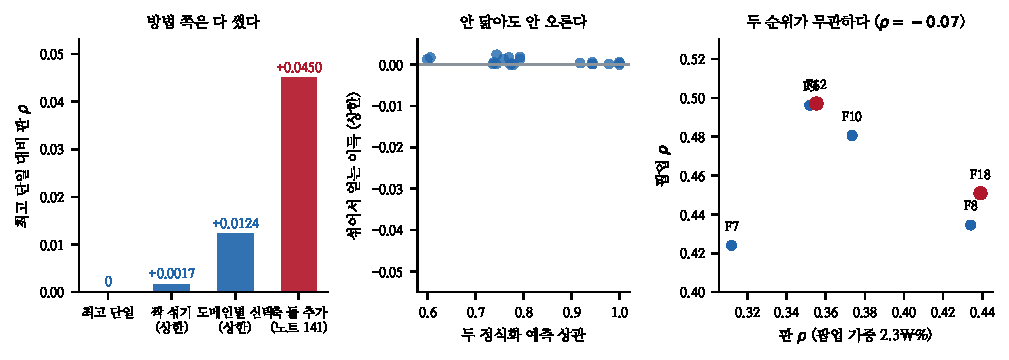
\includegraphics[width=\textwidth]{figs/blend.pdf}
\caption{왼쪽 --- 방법으로 살 수 있는 것과 축으로 산 것. 가운데 --- 안
닮은 짝도 안 오른다. 오른쪽 --- 팝업 순위와 판 순위가 무관하다.}
\end{figure*}

\section{어느 짝을 섞어도 안 오른다}

\begin{table}[t]
\centering\tsize
\caption{짝 섞기. 가중치는 검정 집합에서 최적으로 --- \emph{상한}이다.}
\begin{tabular}{lrrrr}
\toprule
& 상관 & 절반 & 최적 & 이득 \\
\midrule
F10$+$F8 & .744 & $+$.4244 & $+$.4364 & $+$.0024 \\
F7$+$F8 & .605 & $+$.4084 & $+$.4358 & $+$.0017 \\
F10$+$F18 & .769 & $+$.4297 & $+$.4408 & $+$.0017 \\
F7$+$F18 & \textbf{.599} & $+$.4109 & $+$.4404 & $+$.0013 \\
F6$+$F12 & \textbf{.999} & $+$.3558 & $+$.3559 & $+$.0006 \\
\bottomrule
\end{tabular}
\end{table}

\claimx{\textbf{최고 단일을 넘기는 것이 4/21이고 최대 초과가
$+$0.0017이다.} 그것도 가중치를 검정 집합에서 고른 상한이다 --- 정직한
절차로는 이만큼도 못 받는다.}{이득이 나오는 가중치가 전부
$w{=}0.05\sim0.15$다. 약한 모형을 아주 조금 타는 모양은 신호가 아니라
검정 집합에 맞춘 흔적이다.}

\claimx{\textbf{안 닮아도 안 오른다.} 예측 상관이 제일 낮은 짝(F7 대 F18,
$+$0.599)의 이득이 $+$0.0013이다. 노트 147이 짝 sd 0.0140을 보고 ``다르니
섞을 자리가 있다''고 했는데, \emph{다르게 틀리는} 것과 \emph{서로 보완하는}
것은 다르다.}{F6 과 F12 의 예측 상관이 $+$0.999다 --- 공통 축이냐 합집합
축이냐만 다른 두 정식화가 사실상 같은 모형이다. 순위표에 둘을 따로 둘
이유가 없다.}

\section{상한을 더 올려도 축의 4분의 1이다}

\begin{table}[t]
\centering\tsize
\caption{최고 단일($+$0.4391) 대비.}
\begin{tabular}{lrl}
\toprule
& 이득 & \\
\midrule
짝 섞기 (상한) & $+$.0017 & 검정집합 가중치 \\
도메인별 신탁 (상한) & $+$.0124 & 검정집합 선택 \\
\textbf{축 둘 추가} & \textbf{$+$.045} & 노트 141, 정직 \\
\bottomrule
\end{tabular}
\end{table}

\claimx{\textbf{방법 쪽은 다 썼다.} 도메인마다 최고 정식화를 검정 집합을
보고 고르는 --- 절대 못 하는 --- 신탁이 $+$0.0124다. 축 두 개가 $+$0.045였다.
\textbf{못 하는 것을 다 해도 이미 한 것의 4분의 1이다.}}{게다가 노트 139가
도메인별 선택을 안쪽 창으로 해 보니 여섯 중 셋에서 순위 상관이 음수였다 ---
신탁의 반대로 고르는 일이 흔하다.}

\section{그런데 판이 고르는 것이 팝업이 아니다}

\begin{table}[t]
\centering\tsize
\caption{도메인별 $\rho$. 진하게가 그 도메인의 최고.}
\begin{tabular}{lrrrrr}
\toprule
& 몫 & F6/F12 & F10 & F8 & F18 \\
\midrule
웹툰 & 27.3\% & .243 & .250 & .342 & \textbf{.358} \\
애니 & 23.2\% & .433 & .413 & \textbf{.485} & .475 \\
모바일 & 16.9\% & .424 & .505 & .551 & \textbf{.566} \\
세계애니 & 11.5\% & .467 & .396 & \textbf{.498} & .494 \\
\textbf{팝업} & \textbf{2.3\%} & \textbf{.497} & .481 & .435 & .451 \\
\bottomrule
\end{tabular}
\end{table}

\claimx{\textbf{팝업 순위와 판 순위의 상관이 $-$0.071이다.} 판의 1 · 2위
(F18 · F8)가 팝업에서는 5 · 6위이고, 판의 4 · 5 · 6위(F12 · F6 · F9)가
팝업의 1 · 2 · 3위다. \textbf{판은 팝업에 관해 아무것도 안 말한다.}}{판이
표본 수 가중이라 그렇다. 웹툰 27\% · 애니 23\% · 모바일 17\%가 챔피언을
고르고 팝업은 2.3\%다.}

\claimx{\textbf{그렇다고 팝업으로 고를 수도 없다.} F12($+$0.497)와
F18($+$0.451)의 차가 $+$0.046인데 $n{=}59$의 짝 반폭이 0.124다(노트 132의
법칙 $1.03\,n^{-0.52}$). \textbf{팝업은 스스로를 못 가른다.}}{두 문장을
합치면 이렇게 된다 --- 지금 챔피언은 팝업에 관해 고른 것이 아니고, 다른
것을 고를 근거도 없다.}

\section{그래서 병목은 하나다}

세 결론이 같은 곳을 가리킨다. 방법을 섞어도 $+$0.0017, 못 하는 선택까지
해도 $+$0.0124, 그리고 판정치는 목표 도메인에 관해 무정보다. 남은 길은
\textbf{축}과 \textbf{팝업 표본} 둘뿐이고, 둘 다 자료 쪽이다.

\begin{table}[t]
\centering\tsize
\caption{남은 것.}
\begin{tabular}{ll}
\toprule
판정치 & 팝업 가중을 올리면 --- 그러면 분산이 커진다 \\
F6·F12 & 상관 .999 --- 순위표에서 하나로 합칠 것 \\
팝업 & 59 → 202 가 상한(노트 132), 339 이 필요 \\
\bottomrule
\end{tabular}
\end{table}

첫 줄이 다음 자리다. 판정치를 표본 수 가중에서 도메인 균등으로 바꾸면
팝업 몫이 2.3\%에서 11\%로 오른다. 그런데 그러면 아이돌($n{=}25$)도 11\%가
되고 판의 분산이 커진다. \textbf{가중을 바꾸는 것은 순위를 바꾸는 결정이니
점수를 보고 고르면 안 된다} --- 자료의 성질로 정해야 한다.

\end{document}
